\subsubsection{Evaluation verfügbarer Produkte}
\label{sec:produkt-eval}

\paragraph{Auswahl der \ac{waf}-Anwendung}


\paragraph{Verwundbare Anwendungen}

\subsubsection{Labor-Umgebung}

Die in Kapitel \ref{sec:inhalte} beschriebenen Inhalte sollen in einem Praxisnahen Umfeld vermittelt werden.
Dazu kommt nach den Abwägungen aus Kapitel \ref{sec:produkt-eval}, die \ac{waf} ModSecurity zum Einsatz.
Die zu diesem Zweck vorgesehene Laborumgebung muss einige Kriterien erfüllen:
\begin{description}
    \item[Einheitliches Deployment:] Der Ausgangspunkt der Lerneinheiten muss reproduzierbar und wiederholbar sein. 
    Bei wiederholten Durchführungen der Übungen soll es einfach sein den Lernenden ohne zusätzlichem manuellen Konfigurationsaufwand eine Laborumgebung zu übergeben. 
    Diese Laborumgebung muss Platform-unabhängig aufgebaut sein und auf Windows, MacOS unf Linux genutzt werden können.
    \item[Modifizierbarkeit der Anwendungen:] Um in den Lerneinheiten grundlegende Techniken zu übermitteln, ist es notwendig vorkonfigurierte Funktion der ModSecurity \ac{waf} entfernen zu können und den JuiceShop mit Daten zu versehen um eine automatisierte Überprüfung zuu ermöglichen.
    Dies muss automatisiert und auf einem einheitlichen Weg erfolgen können.
    \item[Bekannte Technologien:] Der Fokus der Lerneinheiten liegt auf dem Erlernen der Technik und Funktion einer \ac{waf}. 
    Um einen Einstieg möglichst direkt zu gestalten sollen hierfür Technologien zum Einsatz kommen, die den Lernenden schon bekannt sind und keinen zusätzlichen Lernaufwand erzeugen.
    \item[Komplexe Netzwerkumgebungen:] Da die verschiedenen Anwendungen in der Laborumgebung über Netzwerkkommunikation miteinander kommunizieren, muss es möglich sein automatisiert virtuelle Netzwerke zu erzeugen.
\end{description}

Um den oben genannten Anforderungen möglichst genau zu entsprechen, wird als Teil der Thesis die in Abbildung \ref{fig:lab} schematisch dargestellte Laborumgebung erstellt.

\begin{figure}[!hbt]
    \centering
    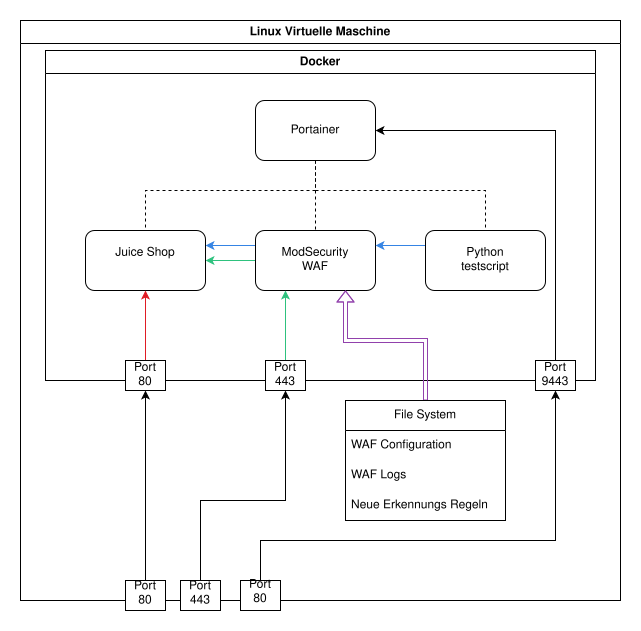
\includegraphics[width=0.9\textwidth]{./images/lab-setup.png}
    \caption{Aufbau der Laborumgebung}
    \floatfoot{Quelle: Eigene Darstellung}
    \label{fig:lab}
\end{figure}

Die Containervirtualisierungsumgebung Docker wird als Deployment-Umgebung verwendet.
Diese ermöglicht es isolierte Ausführungsumgebungen für die Anwendungen zu erzeugen.
Der Aufbau dieser Umgebungen lässt sich mittels einer Konfigurationsdatei genau beschreiben und wiederholbar ausrollen.
Innerhalb der Umgebungen lassen sich virtuelle Netzwerke anlegen um Netzwerkkommunikation vom Host zu isolieren.
Dadurch lässt sich festlegen, wie und welche der einzelnen Anwendungen (Container) untereinander kommunizieren können.
Außerdem können Dateien oder Ordner aus dem Host-Dateisystem in den Container übergeben werden.
Dies ermöglicht es Konfigurationsdateien zur Verfügung zu stellen um die Container zu modifizieren, die sonst \textit{Stateless} sind und nicht vorkonfiguriert ausgeliefert werden.
Im Gegensatz zu virtuellen Maschinen greift die Containervirtualisierungsumgebung direkt auf die Mittel des Host-Betriebssystem zu und benötigt dadurch deutlich weniger Rechenaufwand.\\

Wie in Abbildung \ref{fig:lab} dargestellt, werden in der Laborumgebung vier Container betrieben:

\begin{description}
    \item[ModSecurity \ac{waf}:] Der Hersteller, der in der Laborumgebung verwendeten \ac{waf}: \textit{ModSecurity}, stellt sein Produkt auch in Form eines Docker-Containers zur Verfügung. 
    Diese wird jedoch in modifizierter Form genutzt.
    Um die Lerninhalte zu vermittel muss die große Anzahl vorkonfigurierter Regeln, mit denen die \ac{waf} ausgeliefert wird um den Betrieb zu ermöglichen, entfernt werden.
    An dessen Stelle wird ein Verzeichnis aus dem Host-Dateisystem durchgereicht, in dem die Lernenden eigene Konfigurationen Platzieren können.
    Daneben werden, um das Debugging zu ermöglichen, die Log-Dateien aus der \ac{waf} im Host-Betriebssystem zur Verfügung gestellt.
    
    \item[Juice Shop:] Dieser wird in Version 16.0.0 verwendet, da der Hersteller (OWASP) die Anwendung regelmäßig verändert.
    Durch die Verwendung der neuesten Version könnten Challenges verloren gehen, die für die Durchführung der Aufgaben notwendig wäre.
    Auch diese Anwendung wird modifiziert.
    Es werden Daten hinterlegt und Nutzeraccounts angelegt.
    Diese ermöglichen es mittels eines automatischen Kontroll-Scripts die Konfiguration der \ac{waf} zu überprüfen.
    Die genauen Änderungen werden in den Sub-Kapiteln von Kapitel \ref{sec:learnings} im Detail beschrieben.

    \item[Python Test-Script:] Dieser Container enthält ein Python Skript, das es den Lernenden mittels des Unittest-Frameworks \textit{Pytest} ermöglicht, die erarbeiteten Lösungen zu überprüfen.
    Das Skript schickt \ac{http}-Requests durch die \ac{waf} und evaluiert die Antworten, um den Lernenden Rückmeldung über den Erfolg ihrer Konfiguration zu geben.
    Die jeweilige Funktion wird in den Sub-Kapiteln von Kapitel \ref{sec:learnings} im Detail beschrieben.

    \item[Portainer:] Die Anwendung \textit{Portainer} ermöglicht es eine Docker Umgebung mittels einer Grafischen Oberfläche zu verwalten.
    In der Laborumgebung kann sie genutzt werden um die Laborumgebung zu bedienen ohne sich tiefer mit der Funktion von Docker auseinander setzen zu müssen.
    Zwar können die Lernenden dies auch über das Docker Kommandozeilen-Interface tun, jedoch wird dies als eine vermeidbare Hürde betrachtet, die den Einstieg erschweren könnte.
    Die grafische Oberfläche soll unter anderem genutzt werden um den \ac{waf}-Container nach einer Konfigurationsänderung neu zu starten und mit dem Test Skript zu interagieren. 
\end{description}

Aus den oben genannten Containern ergeben sich einige Netze, die im Hintergrund existieren müssen.
So ist es notwendig, dass eine Verbindung von dem Python-Test-Container zur \ac{waf} und von dieser zum Juice Shop aufgebaut werden kann.
Hierfür werden separate Docker-Netzwerke erstellt die an den Containern angeschlossen sind.
Um den Nutzern eine Interaktion mit den Containern zu ermöglichen werden einige Ports aus der Docker-Umgebung freigegeben:

\begin{itemize}
    \item Die ungesicherte Weboberfläche des Juice Shops (Port 80 [\ac{http}])
    \item Die, durch die \ac{waf} gesicherte, Weboberfläche des Juice Shops (Port 443 [\ac{https}])
    \item Das Management Interface der Portainer-Anwendung (Port 9443 [\ac{https}])
\end{itemize}

Durch die oben beschriebene Docker Umgebung sind Anforderungen an die Laborumgebung wie dem \textit{einheitlichen Deployment} und der \textit{Modifizierbarkeit der Anwendungen} bereits erfüllt.
Es ergeben sich jedoch auch einige Herausforderungen:

\begin{itemize}
    \item Docker ist zwar als Cross-Platform Anwendung konzipiert.
    Es stehen Versionen für die drei gängigen Betriebssysteme Windows, MacOS und Linux zur Verfügung.
    Jedoch bauen die verwendeten Container hauptsächlich auf Linux auf.
    In der Theorie sollte dies zu keinen Problemen führen, da Docker in der Lage ist nicht Platform-Native Container auf sich unterscheidenden Betriebssystemen auszuführen, jedoch kann ein solcher Aufbau durchaus zu unvorhergesehenen Problemen führen.
    \item Ein weiteres Problem ist, dass durch das Durchreichen von Dateien zwischen Container und dem Host-Dateisystem zusätzlicher Konfigurationsaufwand für die Nutzer entsteht.
\end{itemize}

Um diese Probleme zu mittigieren wird die Laborumgebung als Linux Virtuelle Maschine ausgeliefert.
In dieser ist eine Docker-Umgebung vorinstalliert und die Container und Netzwerke bereits präsent und werde automatisiert gestartet.
Dies ermöglicht die Auslieferung mittels einer VM-Datei, in der die Konfigurationen schon an einer einheitlichen Stelle enthalten sind.
Lernende müssen zur Nutzung also nur eine Virtuelle Maschinen auf ihren Rechnern importieren und mittels eines Virtuellen Netzwerk Interface auf die Weboberflächen zugreifen.
Die Konfiguration der \ac{waf} findet in Textdateien statt, die sich in der Virtuellen Maschine befinden.
Der Zugriff auf diese ist mit dem Text-Editor Visual Studio Code der Firma Microsoft vorgesehen, da dieser eine SSH Erweiterung hat die es mit geringen Konfigurationsaufwand ermöglicht Dateien auf entfernten Servern oder in Virtuellen Maschinen zu bearbeiten.

Die Nutzung der Laborumgebung werden durch diese Maßnahmen als einfach genug beurteilt um einen schnellen Einstieg zu ermöglichen.
Die Konfigurationen, die vorgenommen werden müssen, werden in der ersten Lerneinheit (Kapitel \ref{sec:lerneinheit1}) beschrieben.
Es steht den Lernenden frei weitere oder andere als die beschriebenen Technologien zu verwenden, um mit der Laborumgebung zu interagieren.
Diese können im Rahmen dieser Thesis und den Aufgabenstellungen jedoch nicht berücksichtigt werden.

\pagebreak